\chapter{Task Hyper-parameters Matter}
\label{ch:envparams}

Plenty of effort in reinforcement learning has been spent on finding better or faster algorithms that can solve any algorithm as a black box. However, we \red{should I say I?} believe that the design of the character and the tasks can be in some cases far more important in achieving superior results \red{what does good refer to here?} than the algorithm itself. In other words, making the problem itself easier to solve can be easier than finding an algorithm that can solve harder problems. To demonstrate this simple observation in this chapter we will be looking at what we call "task hyper-parameters" as opposed to algorithm hyper-parameters. In \autoref{sec:params_torque} we will be looking at the effects of choosing higher/lower torque limits and we will show that a simple torque limit curriculum can help achieve not just better results but to get there more reliably. In \autoref{sec:params_ts} we will be looking at how the choice of control time-step can effect the control/planning trade-off \red{no results yet}. Lastly, in \autoref{sec:params_residual} we will look at how adding a simple residual action to the controller effects both the learning speed as well as the quality of the motion.


\section{The Effect of Torque Limits}
\label{sec:params_torque}

In order to measure the strength of a person we can measure the strength of its muscles. Similarly we can measure the strength of a robot by measuring the strength of its motors. Since robots do not get tired it suffices to measure the maximum force its motors can apply. Better yet, we can measure the maximum amount of torque that each motor can apply since torque rather than force does not depend on the moment of arm at the output \red{don't think I explained that well}. Therefore for robots and simulated characters modeled after them it is important to have the correct \textit{torque limit} which describes the strength of the motor. Having higher or lower torque limits therefore can have serious implications on what the agent can or cannot do and how "easy" it would be \red{should I describe easy?}.


\red{talk about how lower torque limits is more desirable.}


\subsection{Torque Limit Baseline Experiments}
We can demonstrate the basic idea using a robotic environment and a simple walking task which can later on be used as a baseline. Therefore we choose an environment called the \textit{Walker2D} from the Roboschool package \footnote{\url{https://github.com/openai/roboschool}} and modify it to have a variable torque limit. This environment simulates a simplified bipedal character whose movements are constrained to a 2D plane. The simulation is done using PyBullet \footnote{\url{https://pybullet.org/}} which is a Python interface for the Bullet3 physics engine. The task is simply to walk forward, that is, make as much forward progress as possible in the x-axis. However, the reward function also includes terms other than the forward progress to encourage the agent to use less energy and stay alive longer.

You can see the effect of increasing/decreasing the torque limit in \autoref{fig:torque_limit_base}. Not surprisingly the agents that had a higher torque limit achieve a higher reward. However, below a certain point (0.6x and 0.8x torque limit as well as some of the runs with 1.0x) the agent has not learned to make any forward progress, essentially just stands still and avoids early termination.

\begin{figure}
    \centering
    \begin{subfigure}[t]{\textwidth}
        \centering
        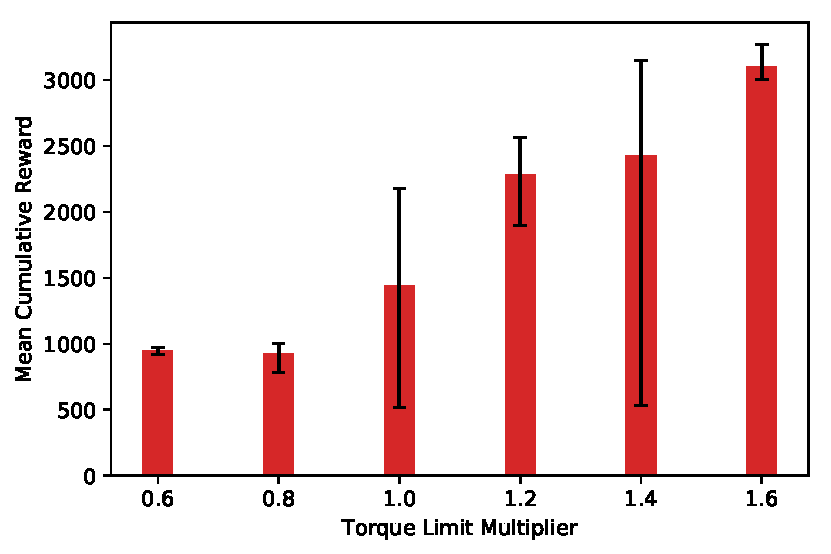
\includegraphics[width=80mm]{img/TorqueLimit_Reward.pdf}
        \caption{Cumulative rewards}
    \end{subfigure}
    \begin{subfigure}[t]{\textwidth}
        \centering
        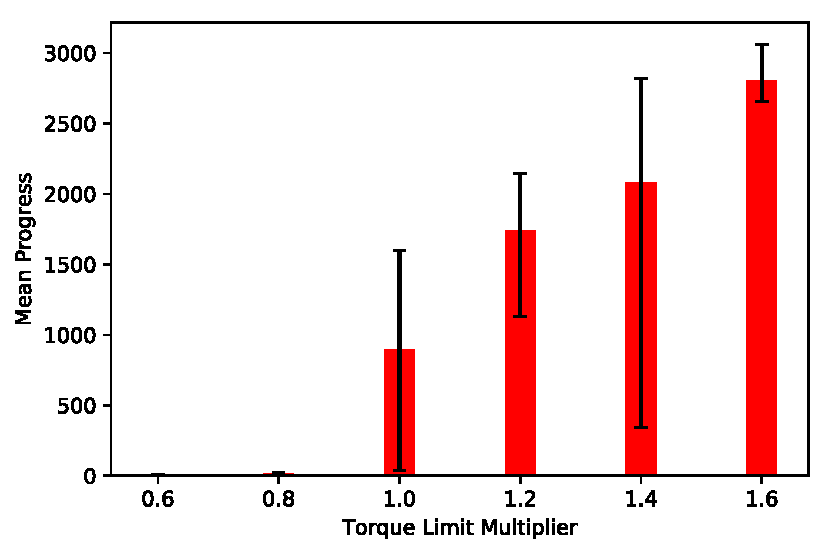
\includegraphics[width=80mm]{img/TorqueLimit_Progress.pdf}
        \caption{Amount of progress in each iteration}
    \end{subfigure}
    \caption{Final performance of the agent with different torque limit levels.}{The error bars reflect the worst and the best performance achieved by the same algorithm over 5 different runs with different seed values.}
    \label{fig:torque_limit_base}
\end{figure}

The results for the default torque limit (1.0x in the same figure) show us something interesting. First, the variance in the results is really high. This is a known problem of reinforcement learning algorithms \cite{rl_that_matters}. More importantly, this hints at the existence of a local optima where the agent does not learn to move (as evident by the zero progress) and just avoids early termination by standing still. \red{maybe I need to explain more why I believe this is a local optima.} Even though the results of training with higher torque limits show variations as well, none of them seem to be stuck in this local optima. Third, the results seem to indicate that it is not possible to learn to walk with the lower torque limits of 0.6 and 0.8. We will shortly see that this is not the case.

\subsection{Torque Limit Curriculum}
If our hypothesis is correct that the agents are getting stuck in a local optima in lower torque limits, it may be possible to get a better controller simply by using a better initialization and the higher torque limit agents though operating in a slightly different regime can be a good starting point. This leads us to use \textit{curriculum learning} \cite{Bengio:2009:CL:1553374.1553380}.

Curriculum learning is motivated by how humans and animals learn and is based on the idea of learning gradually from simple concepts to more difficult ones. In this approach, instead of training on the most difficult version of the problem, the training is divided into multiple stages where the first stage is a simplified version of the problem and task becomes more difficult at each stage until the last stage which is the original problem to be solved.

Since tasks with a higher torque limit seem to be easier to solve, we can define a curriculum where the agent first sees high torque limit environments but gradually the limit is lowered until it matches our target.


\section{The Effect of Control Time-step}
\label{sec:params_ts}

\section{Residual Control for Imitation}
\label{sec:params_residual}
